\documentclass[journal]{IEEEtran}
\usepackage{graphicx}  % Written by David Carlisle and Sebastian Rahtz
\usepackage{amsmath}
\usepackage{color}
\hyphenation{op-tical net-works semi-conduc-tor IEEEtran}
\def\le{\left}
\def\ri{\right}
\def\nnnl{\nonumber\\}
\def\um{\,\mu\mathrm{m}}
\def\comment#1{{\sf #1\/}} 
% paper title
\begin{document}
\title{A Simulation Circuit to Characterize Transistors}
\author{Christoph Maier~\IEEEmembership{Member,~IEEE}% <-this % stops a space
\thanks{Copyright (c) 2014 under Creative Commons
Attribution-NonCommercial-ShareAlike 4.0 International (CC BY-NC-SA 4.0) license.}}%
%~\ref{http://creativecommons.org/licenses/by-nc-sa/4.0/}}% <-this % stops a space
\maketitle
\begin{abstract}\boldmath
I present a simple simulation schematic to extract transistor parameters relevant for analog circuit design:
transconductance~$g_m$, transconductance per current~$g_m/I_d$, voltage gain~$g_m/g_o$, 
and input referred noise~$v_n$.
\end{abstract}


%\begin{IEEEkeywords}
%\ldots
%\end{IEEEkeywords}

\IEEEpeerreviewmaketitle
%%
\section{The circuit}
%%
\begin{figure}[h]
\centering
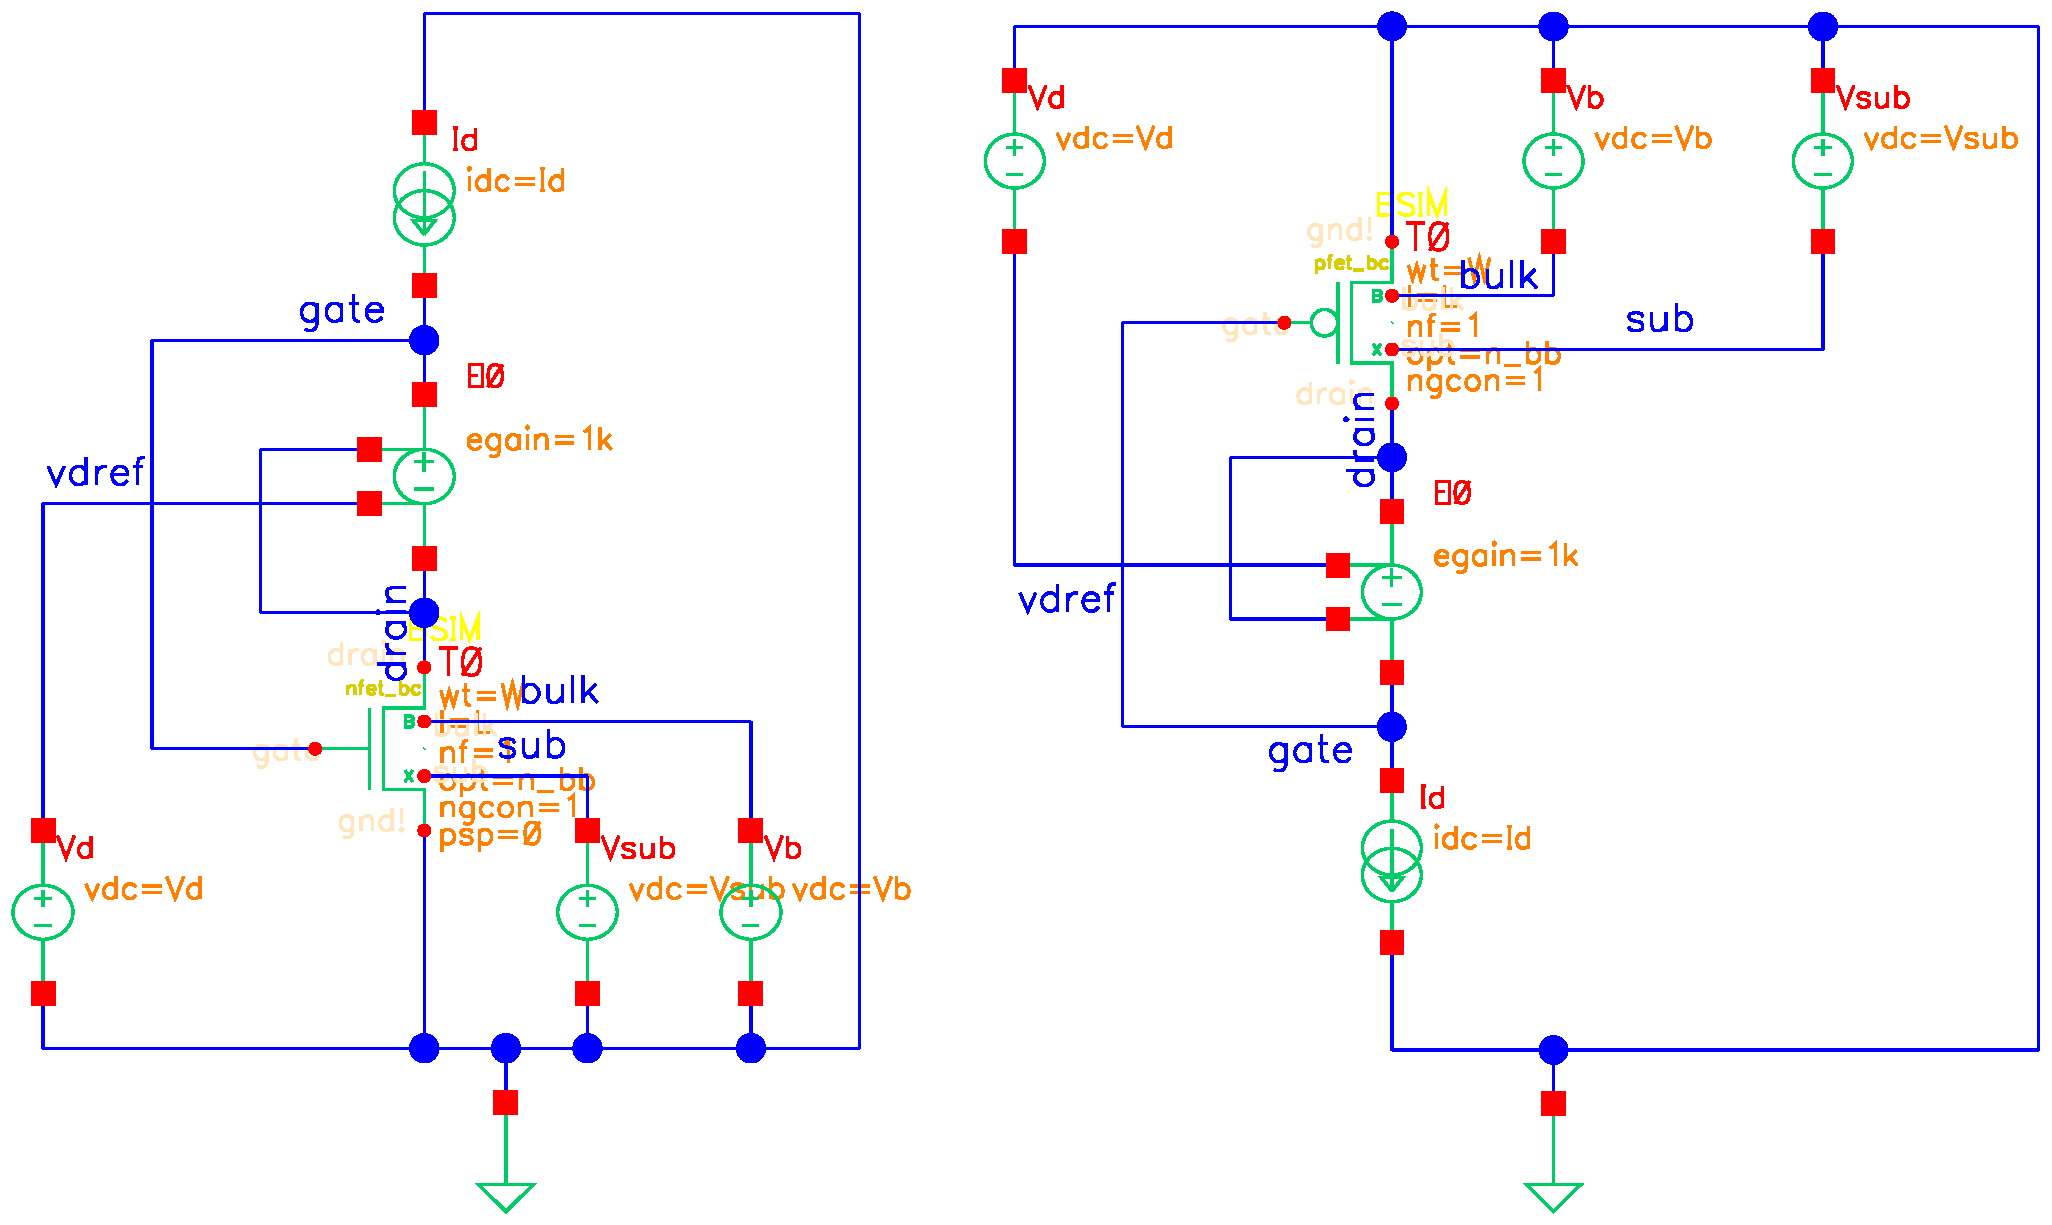
\includegraphics[width=1.0\columnwidth]{figures/mostest_fb.pdf}
\caption{Simulation schematics to characterize MOSFETs}
\label{fig:schematics}
\end{figure}
%
The main design parameters for dimensioning MOSFETs are their drain current~$I_d$, 
which controls transconductance, 
and the drain-to-source voltage~$V_{ds}$, which controls output conductance~$g_o$.
However, the operating point of the transistor is controlled mostly by the gate-to-source voltage~$V_{gs}$.

I solve this by regulating the gate voltage by a feedback loop that adjusts $V_g$ 
to set the drain voltage $V_d$ to a reference $V_{d,ref}$ 
by an ideal voltage controlled voltage source (VCVS). 
The schematics for the NMOS and PMOS simulation circuits are shown in Figure~\ref{fig:schematics}. 

Kirchhoff's Current Law yields the small-signal equations
\begin{IEEEeqnarray}{c}
I_d = g_m V_g + g_o V_d \label{eqn:KCL}\\
V_g = V_d + A \le(V_d - V_{d,ref}\ri) \nonumber
\end{IEEEeqnarray}
which lead to
\begin{equation}\label{eqn:Vg}
V_g = \frac{I_d-g_o\,V_{d,ref}\,A/\le(1+A\ri)}{g_m + g_o/\le(1+A\ri)}
\end{equation} 
and
\begin{equation}\label{eqn:Vd}
V_d = \frac{I_d+A\,g_m\,V_{d,ref}}{\le(1+A\ri) g_m + go}\,.
\end{equation} 

In the ideal case of $A\rightarrow\infty$, 
\begin{equation}\label{eqn:Vg_ideal}
V_g = \frac{I_d-g_o\,V_{d,ref}}{g_m}
\end{equation} 
and
\begin{equation}\label{eqn:Vd_ideal}
V_d = V_{d,ref}\,.
\end{equation} 

\section{Parameter extraction}
%%
\subsection{Transconductance}
%
The transconductance $g_m$ as function of drain current can be obtained 
by sweeping $I_d$ for fixed $V_d$, as 
\begin{equation}\label{eqn:gm}
1/\le(\frac{\partial V_g}{\partial I_d}\ri) = g_m+g_o/\le(1+A\ri) 
\overset{A\rightarrow\infty}{\approx} g_m\,.
\end{equation}

\subsection{$g_m/I_d$}
%
The specific transconductance $g_m/I_d$ is a useful design parameter 
for setting the bias point of a transistor. $g_m/I_d$ is maximal in subthreshold operation. 
It is obtained by sweeping $I_d$ for fixed $V_d$ and calculating
\begin{equation}\label{eqn:gm_over_Id}
1/\le(\frac{\partial V_g}{\partial I_d}\,I_d\ri) = \frac{g_m+g_o/\le(1+A\ri)}{I_d}
\overset{A\rightarrow\infty}{\approx} \frac{g_m}{I_d}\,.
\end{equation}

\subsection{$g_m/g_o$}
%
While $g_m$ or $g_m/I_d$ is the most important design criterion for dimensioning a transistor,
the next most important criterion is setting the output conductance $g_o$. 
With the circuits in Figure~\ref{fig:schematics}, 
the intrinsic voltage gain $g_m/g_o$ can be extracted by sweeping $V_{d,ref}$ for constant $I_d$.
\begin{equation}\label{egn:gm_over_go}
-\le(\frac{\partial V_d}{\partial V_{d,ref}}\ri)
/\le(\frac{\partial V_g}{\partial V_{d,ref}}\ri)
= \frac{\frac{A\,g_m}{\le(1+A\ri)g_m+g_o}}{\frac{A\,g_o}{\le(1+A\ri)g_m+g_o}} 
= \frac{g_m}{g_o} \,.
\end{equation}

\subsection{Noise}
%
Due to the feedback in the schematic in Figure~\ref{fig:schematics},  
the input referred noise of the transistor can be observed directly at the regulated gate. 
When a term for input referred noise is added to Equation~\ref{eqn:KCL}, 
\begin{IEEEeqnarray}{c}
I_d = g_m (V_g+v_n) + g_o V_d \label{eqn:noisyKCL}\\
V_g = V_d + A \le(V_d - V_{d,ref}\ri) \nonumber
\end{IEEEeqnarray}
the effect of the noise voltage $v_n$ on the gate voltage $V_g$ is 
\begin{equation}\label{eqn:noiseVg}
\frac{\partial V_g}{\partial v_n} = -\frac{1}{1+\frac{g_o}{\le(1+A\ri)g_m}}
\end{equation}
and 
\begin{equation}\label{eqn:gatenoise}
v_n = -\le(1+\frac{g_o}{\le(1+A\ri)g_m}\ri)V_g 
\overset{A\rightarrow\infty\atop g_o\ll g_m}\approx -V_g \,.
\end{equation}
The input referred noise of the transistor can be read 
by setting the output node of the noise to $V_g$.
\end{document}


